\section{Decomposition-based Solution Approaches}
\label{section:solutionmethodology}
The aircraft maintenance scheduling and assignment problem Eqs.~\eqref{eq:ObjDaystogo} to \eqref{eq:JointBinary4} presented in Section~\ref{Problem_definition_formulation} is a mixed integer program, which can be solved with a commercial solver when the problem scale is limited. However, this problem has a very large scale for realistic instances. This is evident as both the number of variables and constraints grow rapidly as the problem size increases. For instance, the number of variables $x_{wj}^t$ increases with the number of tuples $|W|$, number of stations $|J|$, and number of days in the planning horizon $|T|$. Similarly, the number of constraints also grows with the number of stations and/or the planning horizon length. This observation motivates us to decompose a large-scale scheduling and assignment problem into smaller and more manageable sub-problems. Specifically, we seek to explore two decomposition strategies: (1) separating assignment from scheduling and (2) temporal decomposition.

In Section~\ref{sec:SchedulingThenAssign}, we first describe a scheduling-first-assignment-second solution approach; in Section~\ref{sec:tempDecomp}, we seek to achieve the temporal decomposition with a rolling horizon approach.

 


% \subsection{Scheduling-then-Assigning Approach}
\subsection{Sequential Heuristic (SH) Approach}
\label{sec:SchedulingThenAssign}
In the base formulation Eqs.~\eqref{eq:ObjDaystogo} to \eqref{eq:JointBinary4}, we jointly optimize the scheduling and assignment decisions. We now explore a decomposition-based heuristic by sequentially optimize scheduling and assignment decisions. In the scheduling stage, no information about individual maintenance stations is available; only the aggregated capacity parameters are known. In the assignment stage, all optimization decisions made during the scheduling stage are known as inputs and the new decision is to assign tuples to stations day by day.

Table~\ref{tab:notation_tabDecomp} shows some additional notation used in the decomposition approach. Note that the notation in Table~\ref{tab:notation_tab} remains applicable.


% \usepackage{array}


\begin{table}[ht]
\centering
\caption{Notation used in the scheduling-only problem}
\label{tab:notation_tabDecomp}
\begin{tabular}{lp{16cm}} 
\toprule
\multicolumn{2}{l}{\textit{Parameters}} \\ 
\hline
$\bar{P}_{s}^t$ & Maximum number of aircraft of subfleet type $s$ that can be routed to any maintenance stations on day $t$, $\bar{P_{s}^t} =\sum_{j\in J}P_{sj}^t$ \\
$\bar{H}^t$ & Maximum man-hours available on day $t$, $\bar{H}^t =\sum_{j\in J}H_j^t$ \\
$\bar{Q}^t$ & Number of distinct aircraft that a station can handle on day $t$ for maintenance, $\bar{Q}^t =\sum_{j\in J}Q_j^t$ \\
$\bar{U}^t$ & Maximum number of phase checks that can be accomplished on day $t$, $\bar{U} =\sum_{j\in J}U_j^t$ \\
$R^\prime$ & Maximum number of phase checks that can be performed simultaneously on a given aircraft at any station daily, $\hat{R} = \max_j\left\{R_j^t\right\}$ \\
$e_i^t$ & A binary parameter to indicate if at least one of the maintenance stations that can complete multiple phase check has nonzero station access for aircraft $i$ on day t \\
$\bar{A}^t$ & Maximum number of A-checks that can be accomplished on day $t$, $\bar{A} =\sum_{j\in J} A_j^t$ \\
$\bar{I}$ & Set of aircraft needing phase checks \\ 
$\bar{I_s}$ &  Set of all aircraft of subfleet type $s$ needing phase checks \\ 
\hline
\multicolumn{2}{l}{\textit{Decision Variables}} \\ 
\hline
$x_w^t$ & A binary variable to be 1 if tuple $w$ is scheduled for day $t$ \\
$y_w^t$ & Days-to-go for aircraft $i$ for check $k$ on day $t$ \\
$z_i^t$ & A binary variable to be 1 if aircraft $i$ is scheduled for maintenance on day $t$ \\
$\hat{\psi}_i^t$ & A binary variable to be 1 if One-C Phase Check is scheduled on day $t$ for aircraft $i$ \\
$\breve{\psi}_i^t$ & A binary variable to be 1 if Two-C Phase Check is scheduled on day $t$ for aircraft $i$ \\ \bottomrule
\end{tabular}
\end{table}
% \newpage

By dropping aircraft-to-station assignment decisions from the joint optimization problem Eqs.~\eqref{eq:ObjDaystogo} to \eqref{eq:JointBinary4}, we have the following scheduling-only problem (SOP) using additional notation in Table~\ref{tab:notation_tabDecomp}:
\begin{flalign}
\text{(SOP)} \quad	\min_{\left\{x_{w}^t, y_w^t,z_i^t,\hat{\psi}_i^t,\breve{\psi}_i^t \right\}}  \quad  \quad  &  \sum_{w \in W}\sum_{t \in T} \gamma^t x_{w}^t  \label{eq:ObjDaystogoSub} \\
    %Days to go evolution
    \text{s.t.}  \quad \quad &  y_w^1 =\delta_w^0, \quad \forall w \in W \label{eq:initial_day_to_gosub}\\
    & y_w^t \leq y_w^{t-1} - 1 + m_w x_{w}^{t-1}, \quad \forall w \in W, t \in T \setminus \left\{1\right\} \label{eq:statusEvolution-dtgsub} \\
     & y_w^t \ge m_w x_{w}^{t-1}, \quad \forall w \in W , t \in T \setminus \left\{1\right\} \label{eq:statusEvolution-dtgAddedsub} \\
     & y_w^t \ge y_w^{t-1} - 1, \quad \forall w \in W, t \in T \setminus \left\{1\right\}\label{eq:statusEvolution-dtg_2sub} \\
    & 1 \leq y_w^t \leq m_w, \quad \forall w \in W, t \in T  \label{eq:withinLimits_dtgsub} \\
    % Linking x_w^t to z_i^t
    & \sum_{w \in W_i} x_{w}^t \leq M z_i^t, \quad \forall i \in I, t \in T \label{eq:routingDepen_sub}\\
    % station Access
    & \sum_{i \in I_s}z_i^t   \leq  \bar{P}_{s}^t, \quad \forall s \in S,t \in T \label{eq:stationaccess_sub}\\
    % Resource constraints.
    & \sum_{w \in W}l_w x_{w}^t  \leq \bar{H}^t, \quad \forall  t \in T \label{eq:manhourcapacity_sub}\\
    &\sum_{i \in I}z_{i}^t \leq \bar{Q}^t, \quad \forall  t \in T  \label{eq:checkwork_check_capacitysub} \\
    &\sum_{w \in \bar{W}} x_{w}^t\leq  \bar{A}^t, \quad t \in T \label{eq:station_Acheck_capacitysub}  \\
    & \hat{\psi}_i^t +\breve{\psi}_i^t \leq z_i^t, \quad \forall  t \in T, i \in \bar{I}  \label{eq:notsamephasecheckschd} \\
     & \sum_{w \in\hat{W}_i}x_{w}^t  \leq R^{\prime}  \hat{\psi}_i^t, \quad \forall  t \in T, i \in \bar{I}  \label{eq:station_phasecheck_capacityhat} \\
      & \sum_{w \in\breve{W}_i}x_{w}^t  \leq R^{\prime} \breve{\psi}_i^t, \quad \forall  t \in T, i \in \bar{I}  \label{eq:station_phasecheck_capacitybreve} \\
    & \sum_{w \in\hat{W}_i}x_{w}^t  \leq (R^{\prime} - 1)e_i^t + 1, \quad \forall  t \in T, i \in \bar{I}  \label{eq:station_phasecheck_capacityhat2} \\ 
    & \sum_{w \in\breve{W}_i}x_{w}^t  \leq (R^{\prime} - 1)e_i^t + 1 , \quad \forall  t \in T, i \in \bar{I}  \label{eq:station_phasecheck_capacitybreve2} \\
    &  \sum_{i \in \bar{I}}\left(\sum_{w \in \hat{W_i}} x_{w}^t + \sum_{w \in \breve{W_i}} x_{w}^t\right)  \leq \bar{U}^t,  \quad \forall  t \in T \label{eq:phasechecktotal} \\
    & x_{w}^t \in \{0,1\},  \quad \forall w \in W,  t \in T\label{eq:JointBinarysub_xw} \\
    & y_w^t \in R,  \quad \forall w \in W, t \in T \label{eq:JointBinary1sub} \\
    & z_{i}^t \in \{0,1\},  \quad \forall i \in I,  t \in T\label{eq:JointBinarysub_zi} \\
    & \hat{\psi}_i^t \in \{0,1\}, \quad \forall t \in T, i \in \bar{I} \label{eq:oneCsched} \\
    & \breve{\psi}_i^t \in \{0,1\}, \quad \forall t \in T, i \in \bar{I} \label{eq:two2sched}
 \end{flalign} 



The optimization objective Eq.~\eqref{eq:ObjDaystogoSub} minimizes the total discounted maintenance cost. 
Constraint~\eqref{eq:initial_day_to_gosub} initializes the DTG for each tuple $w$. Similar to the joint optimization model, constraints~\eqref{eq:statusEvolution-dtgsub} to \eqref{eq:withinLimits_dtgsub} model the day-to-day evolution of DTG considering the maintenance timing.
Constraint~\eqref{eq:routingDepen_sub} ensures that if aircraft $i$ is not routed for maintenance on day $t$, no tuples in set $W_i$ associated with aircraft $i$ can be scheduled for day $t$.
Constraint~\eqref{eq:stationaccess_sub} ensures that the number of aircraft routed for maintenance on day $t$ is capped for each subfleet type $s$ and day $t$.
Constraint~\eqref{eq:manhourcapacity_sub} ensures that the network-wide man-hour limit is not exceeded on day $t$. 
Constraint~\eqref{eq:checkwork_check_capacitysub} ensures that the maximum number of distinct aircraft that can be maintained on day $t$ is not exceeded. 
Constraint~\eqref{eq:station_Acheck_capacitysub} enforces the A check limit per day.
Constraint~\eqref{eq:notsamephasecheckschd} ensures that only one type of phase checks (i.e., either One-C or Two-C) can be scheduled on day $t$ for aircraft $i$ if aircraft $i$ is routed for maintenance on day $t$. Otherwise, no phase checks of any type can be scheduled.
Constraint~\eqref{eq:station_phasecheck_capacityhat} states that if One-C phase checks are scheduled for aircraft $i$ on day $t$, the limit is $R^{\prime}$. Constraint~\eqref{eq:station_phasecheck_capacitybreve} enforces the same requirement as in constraint~\eqref{eq:station_phasecheck_capacityhat} but for Two-C phase checks. 
Constraint~\eqref{eq:station_phasecheck_capacityhat2} states that at most one One-C phase check can be completed for aircraft $i$ on day $t$, unless $e_i^t = 1$. $e_i^t$ is a binary parameter indicating whether at least one station exists that can accommodate multiple phase checks and has a nonzero station access.
% that indicates whether there exists at least one station capable of accommodating multiple phase checks and also has a nonzero station access. 
When $e_i^t = 1$, the maximum number of phase checks that can be completed daily is $R^{\prime}$. As defined in Table~\ref{tab:notation_tabDecomp}, $R^{\prime} = \max_j\left\{R_j\right\}$, an aircraft $i$ can be routed to one maintenance station at most, the number of phase checks that can be scheduled for aircraft $i$ must be capped at $\max_j\left\{R_j\right\}$.
Constraint~\eqref{eq:station_phasecheck_capacitybreve2} enforces the same requirement but for Two-C phase checks.
Constraint~\eqref{eq:phasechecktotal} enforces the phase check limit per day at the system-level.
Constraints~\eqref{eq:JointBinarysub_xw}, \eqref{eq:JointBinary1sub}, \eqref{eq:JointBinarysub_zi}, \eqref{eq:oneCsched}, and  \eqref{eq:two2sched} together define the domains for the decision variables.

After solving the scheduling-only problem Eqs.~\eqref{eq:ObjDaystogoSub} to \eqref{eq:two2sched}, we know whether tuple $w$ is scheduled for day $t$, indicated by the value of $x_{w}^t$, and if aircraft $i$ is routed for maintenance on day $t$, indicated by the value of $z_{i}^t$. Given the above scheduling decisions, we next determine how those aircraft scheduled for maintenance on day $t$ are assigned to various stations, subject to station-specific capabilities and capacity limits. 

\begin{figure}[htbp]
    \centering
    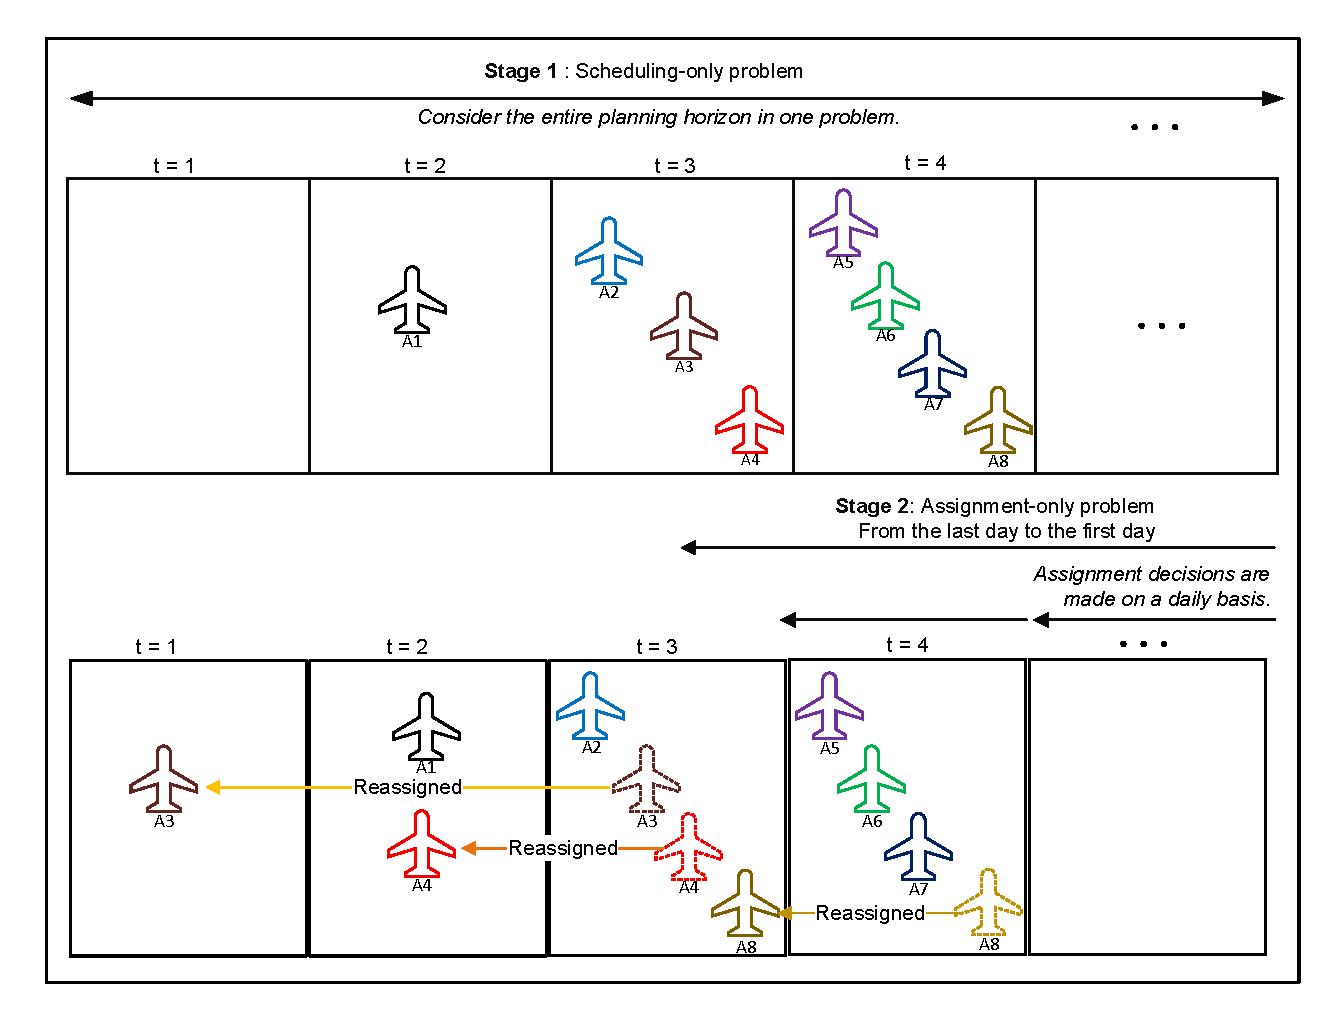
\includegraphics[width=\linewidth]{sequential_heurisicsv3.pdf}
    \caption{Illustration for the sequential heuristic decomposition framework}
    \label{fig:sh-framework}
\end{figure}


For the planning horizon $T$ in the SOP, we solve the assignment-only problem (AOP) daily, starting from the end of the planning horizon, namely Day $|T|$, going backward to the first day, namely Day 1 as shown in Figure~\ref{fig:sh-framework}. Note that not all tuples scheduled for day $t$ can be accommodated. For instance, two A checks are scheduled for a day and the total capacity is sufficient. When those two checks are assigned to two stations, infeasibility arises because one station has sufficient man hours while its station access is zero; the other station has sufficient station access while not having enough man hours. Therefore, it is likely that the aggregated capacity is sufficient while the capacity at the station level is insufficient. When such an infeasibility issue arises, namely, a tuple cannot be accommodated on a scheduled day $t$, we shift it to an earlier day $t-1$. Shifting a scheduled tuple to an earlier date will not cause the DTG to be inadmissible (i.e., dropping below the minimum value of 1).


% \begin{figure}[htbp]
%     \centering
%     \includegraphics[width=\linewidth]{sequential_heurisics.pdf}
%     \caption{Illustration for the sequential heuristic decomposition framework}
%     \label{fig:sh-framework}
% \end{figure}




\begin{table}[ht]
\centering
\caption{Notation used in the AOP}
\label{tab:notation_tabDecomp2}
\begin{tabular}{lp{16cm}} 
\toprule
\multicolumn{2}{l}{\textit{Sets and Indices}} \\ 
\hline
$I^t$ & Set of aircraft routed for maintenance on day $t$ \\
$I_s^t$ & Set of aircraft of a particular subfleet type $s$ routed for maintenance on day $t$, $I_s^t = I_s \cap I^t$ \\
$W^t$ & Set of tuples scheduled for day $t$ \\
$W_i^t$ & Set of tuples scheduled for day $t$ for aircraft $i \in I^t$ \\
$\bar{W^t}$ & Set of A check tuples scheduled for day $t$, $\bar{W^t} \subseteq W^t$ \\
$\hat{W^t}$ & Set of One-C-check tuples scheduled for day $t$, $\hat{W^t} \subseteq W^t$ \\
$\hat{W_i^t}$ & Set of One-C-check tuples scheduled for day $t$ and aircraft $i$, $\hat{W_i^t} \subseteq W^t $ \\
$\breve{W^t}$ & Set of Two-C-check tuples scheduled for day $t$, $\breve{W^t} \subseteq W^t$ \\
$\breve{W_i^t}$ & Set of Two-C-check tuples scheduled for day $t$ and aircraft $i$, $\breve{W_i^t} \subseteq W^t$ \\ 
\hline
\multicolumn{2}{l}{\textit{Parameter}}  \\
\hline
$\phi_{ij}^t$ & A binary parameter indicating whether aircraft $i$ has been routed to station $j$ for maintenance in $\eta + 1$ days from day $t$ \\
$F$ & Penalty for not accommodating a tuple, e.g., 100  \\
\hline
\multicolumn{2}{l}{\textit{Decision Variables}} \\ 
\hline
$\alpha_{wj}^t$ & A binary variable to be 1 if tuple $w$ is assigned to station $j$ for maintenance on day $t$ \\
$\theta_{ij}^t$ & A binary variable to be 1 if aircraft $i$ is routed to station $j$ for maintenance on day $t$ \\
$\hat{\varphi_j}^t$ & A binary variable to be 1 if station $j$ is open for One-C Phase checks on day $t$ \\
$\breve{\varphi_j}^t$ & A binary variable to be 1 if station $j$ is open for Two-C Phase check on day $t$  \\
$\lambda_{w}^t$ & A binary variable to be 1  if a scheduled tuple $w$ is not accommodated on day $t$ \\ 
\hline
\end{tabular}
\end{table}



Hence, with additional notation in Table~\ref{tab:notation_tabDecomp2}, we present the aircraft-to-station assignment-only problem for a given day $t$ as follows:
\begin{flalign}
\text{(AOP)} \quad \min_{\left\{\alpha_{wj}^t, \theta_{ij}^t, \hat{\varphi_j}^t,\breve{\varphi_j}^t, \lambda_{w}^t\right\}} \quad & \sum_{w \in W^t} \sum_{j \in J_w} \beta_{wj} \alpha_{wj}^t + F\sum_{w \in W^t} \lambda_{w}^t\label{eq:ObjAssignment} \\
    \text{s.t.} \quad & \sum_{j \in J_w} \alpha_{wj}^t + \lambda_{w}^t  = 1, \quad \forall w \in W^t  \label{eq:OneStationPerTuple} \\
    & \sum_{w \in W_i^t} \alpha_{wj}^t \leq M \theta_{ij}^t, \quad  \forall i \in I^t, j \in J \label{eq:LinkVisit} \\
    & \sum_{i \in I_s^t} \theta_{ij}^t   \leq  P_{sj}^t, \quad \forall s \in S,j \in J \label{eq:stationaccess_subAssin}\\
    & \sum_{w \in W^t} l_w \alpha_{wj}^t \leq H_j, \quad \forall j \in J \label{eq:StationManhours} \\
    & \sum_{i \in I^t}  \theta_{ij}^t \leq Q_j, \quad \forall j \in J\label{eq:StationCap} \\
    & \sum_{j \in J_i} \theta_{ij}^t \leq 1, \quad \forall i \in I^t \label{eq:OneStationPerAircraft} \\
    & \sum_{w \in \bar{W^t}} \alpha_{wj}^t \leq A_j^t, \quad \forall j \in J \label{eq:StationACheckCapacity} \\
    & \hat{\varphi_j^t} + \breve{\varphi_j^t} \leq 1,  \quad \forall j \in J \label{eq:sub-notsamephasechecktype} \\
    & \sum_{w \in \hat{W^t}} \alpha_{wj}^t \leq U_j^t\hat{\varphi_j^t}, \quad \forall j \in J \label{eq:sub-notsamephasechecktypehat} \\
    & \sum_{w \in \breve{W^t}} \alpha_{wj}^t \leq U_j^t \breve{\varphi_j^t}, \quad \forall j \in J \label{eq:sub-notsamephasechecktypebreve}  \\
    & \sum_{w \in \hat{W_i^t}} \alpha_{wj}^t + \sum_{w \in \breve{W_i^t}} \alpha_{wj}^t \leq R_j^t, \quad \forall i \in I^t, \forall j \in J \label{eq:PhaseCheckPerAircraft} \\
    & \phi_{ij}^t + \theta_{ij}^t \leq 1, \quad \forall i \in I^t, j \in J \label{eq:NoRepeatVisits} \\
    & \alpha_{wj}^t \in \{0,1\}, \quad \forall w \in W^t,  j \in J_w \label{eq:BinaryAssignment} \\
    & \theta_{ij}^t \in \{0,1\}, \quad \forall i \in I^t, j \in J_i \label{eq:AircraftAssignment} \\
    & \hat{\varphi_j^t} \in \{0,1\}, \quad \forall j \in J \label{eq:openOneC} \\
    & \breve{\varphi_j^t} \in \{0,1\}, \quad \forall j \in J \label{eq:openTwoC} \\
    & \lambda_w^t \in \{0,1\}, \quad \forall w \in W^t\label{eq:notassignedtuple}
\end{flalign}

The objective function Eq.~\eqref{eq:ObjAssignment} prioritizes the assignment of tuples to their preferred stations while simultaneously minimizing the total number of tuples that cannot be accommodated on day $t$.
Constraint~\eqref{eq:OneStationPerTuple} ensures that each tuple $w \in W^t$ must be scheduled for maintenance (i.e., $\sum_{j \in J_w} \alpha_{wj}^t = 1$); otherwise, $\lambda_{w}^t = 1$, meaning that tuple $w$ is left unscheduled.  
Constraint~\eqref{eq:LinkVisit} ensures that none of aircraft $i$'s check tuples can be assigned to station $j$ unless aircraft $i$ is routed to station $j$.
Constraint~\eqref{eq:stationaccess_subAssin} is the station access constraint for station $j$.
Constraint~\eqref{eq:StationManhours} is the man-hour constraint.
Constraint~\eqref{eq:StationCap} ensures that the maximum number of aircraft routed to station $j$ is capped at $Q_j$.
Constraint~\eqref{eq:OneStationPerAircraft} ensures that aircraft $i$ must be routed to a compatible station for maintenance.
Constraint~\eqref{eq:StationACheckCapacity} ensures that the number of A-check-tuples assigned to station $j$ does not exceed $A_j^t$. 
Constraint~\eqref{eq:sub-notsamephasechecktype} ensures that at station $j$, we can have only type of One-C phase checks or Two-C phase checks.
Constraint~\eqref{eq:sub-notsamephasechecktypehat} ensures that if station $j$ is open for One-C phase check, then the total number of One-C phase checks assigned to it should not exceed limit $U_j^t$.
Similarly, constraint~\eqref{eq:sub-notsamephasechecktypebreve} enforces the exact requirement but for Two-C checks. 
Constraint~\eqref{eq:PhaseCheckPerAircraft} states that the total number of phase checks performed on aircraft $i$ at station $j$ does not exceed $R_j$.
Constraint~\eqref{eq:NoRepeatVisits} ensures that when an aircraft cannot visit the same station for maintenance within a period of $\eta$ days.
Constraints~\eqref{eq:BinaryAssignment}, \eqref{eq:AircraftAssignment}, \eqref{eq:openOneC},  \eqref{eq:openTwoC}, and \eqref{eq:notassignedtuple} define decision variables as binary.



\subsection{Temporal Decomposition (TD) Approach}
\label{sec:tempDecomp}
In Section~\ref{sec:SchedulingThenAssign}, the overall strategy is to decompose the optimization problem based on the type of decisions (scheduling vs assignment). We next present a different decomposition strategy, which is based on time. The temporal decomposition can be described with a rolling horizon framework, illustrated in Figure~\ref{fig:temp-dec_illustration}. 

\begin{figure}[htbp]
    \centering
    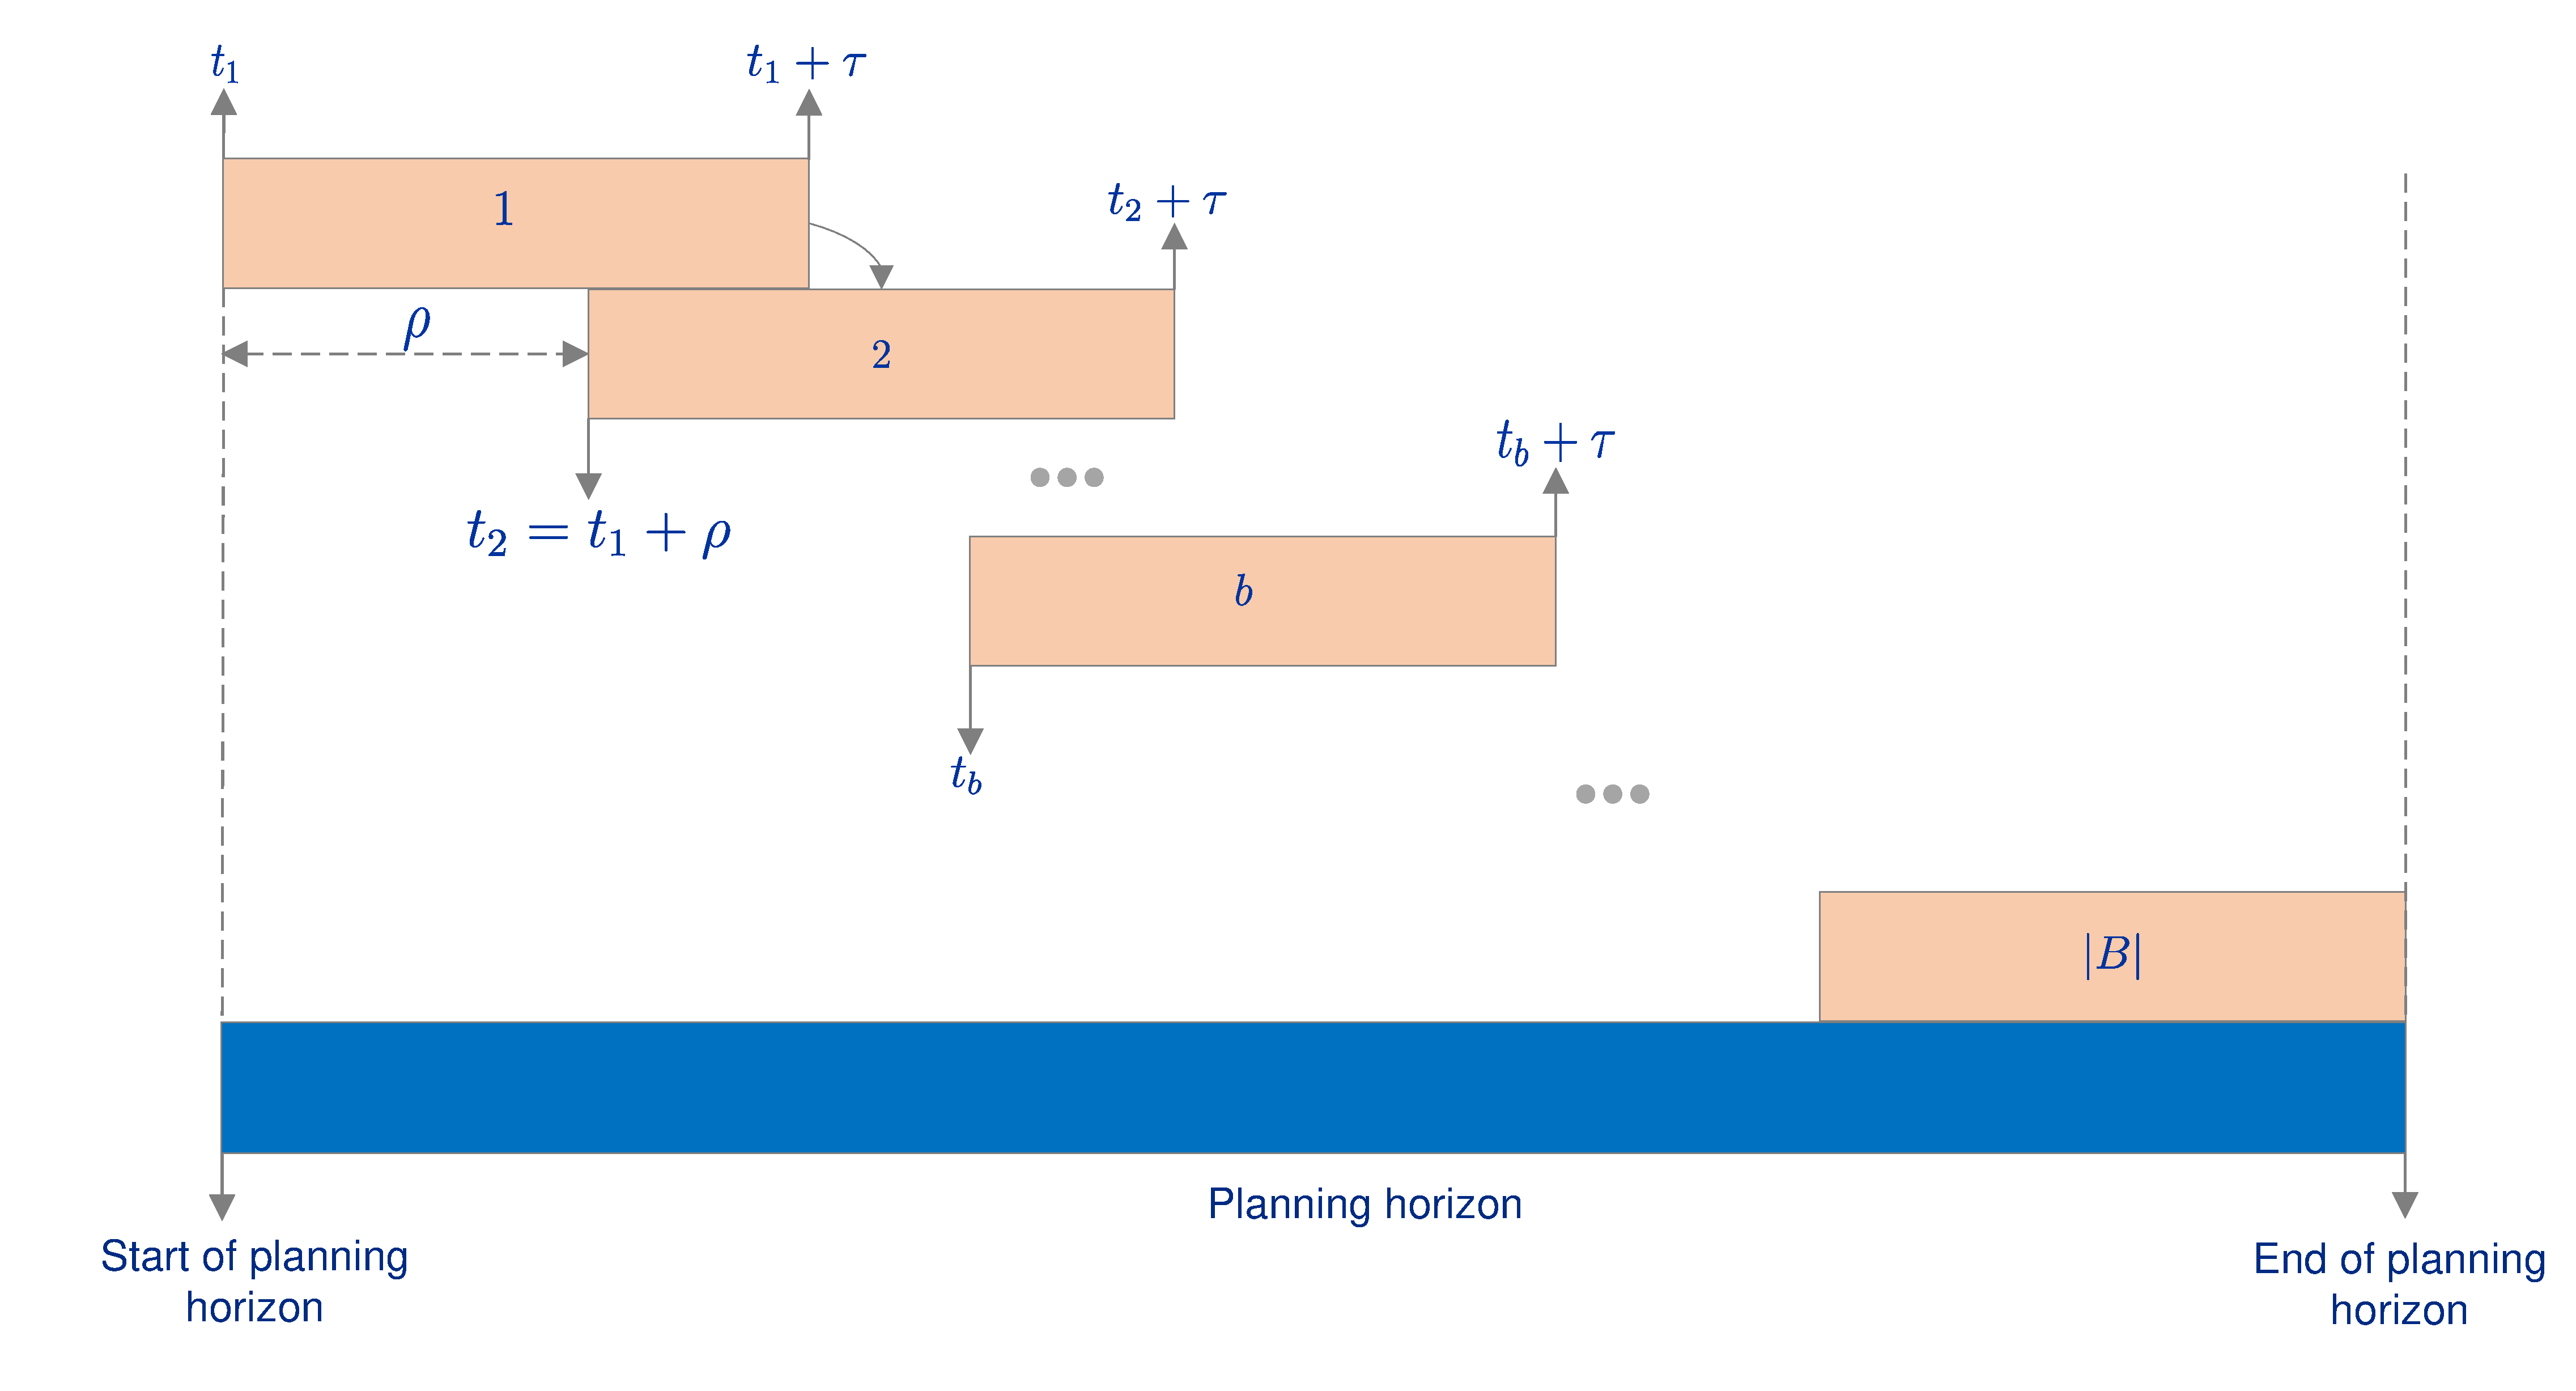
\includegraphics[width=\linewidth]{updated_temporal_decompositionv2.pdf}
    \caption{Illustration for the temporal decomposition framework}
    \label{fig:temp-dec_illustration}
\end{figure}



The original planning horizon $T$ is decomposed into a series of partially overlapping time horizons of equal length $\tau$. Each time horizon $b$ begins at $t_b$ and ends at $t_b + \tau$, where $b \in \{1, 2, \dots, |B|\}$ and $|B|$ is the total number of time horizons. The start time of the immediate next time horizon, namely $b+1$, is $t_b + \rho$, where $\rho$ is the rolling period. As $\rho < \tau$, some overlap between time horizons $b$ and $b+1$ is built in by design. The primary motivation for keeping the overlap between two consecutive time horizons is to address the End-of-Horizon effect described in Proposition~\ref{lem:EndOfHorizon}. We can illustrate this with a simple case where the first horizon covers Day 1 to Day 10, and the second horizon covers Day 11 to Day 20. As there is no overlap between the two horizons, it is possible that for certain tuples, the DTG is 1 on Day 10, while no maintenance is scheduled on Day 10. On Day 11, the DTG would drop to zero for the above said tuples, thus leading to infeasibility issues. 

We next describe how a joint optimization problem $\Delta_b$ is formulated for time horizon $b$. Among all those tuples in $W$, only those tuples meeting $\delta_w^0 \leq t_b + \tau + \epsilon$ are considered in $\Delta_b$, where $\delta_w^0$ is the updated DTG for each tuple $w \in W$ at $t_b$. The formulation Eqs.~\eqref{eq:ObjDaystogo} to \eqref{eq:JointBinary4} is built based on the above stated subset of $W$ and a planning horizon of $t_b$ to $t_b + \tau$. After solving problem $\Delta_b$, we obtain the optimum values of key decision variables, such as $\bar{x}_{wj}^t$, $\bar{y}_w^t$, and $\bar{z}_{ij}^t$. Those planning decisions in the first part of time horizon $b$, namely from $t_b$ to $t_b + \rho$, are finalized; however, those planning decisions in the second part, namely from $t_b + \rho$ to $t_b + \tau$, will be re-optimized in the next time horizon $b+1$. 

With the above described approach, we solve the joint problem for each time horizon sequentially until planning decisions over the entire planning horizon are available.



For each horizon $b$, constraint~\eqref{aircraft_rotation} is defined for the following days in horizon $b$: $t_b, t_b+1,\dots,t_b+\tau-\eta+1$. Constraint~\eqref{aircraft_rotation} defined for day $t$ covers the following period of $\eta$ days: $t, t+1,\dots,t+\eta-1$. However, the aircraft rotation constraint is not enforced for the following $\eta$-day periods consisting of day $t_b$:
\begin{itemize}
    \item $t_b-\eta+1,\dots,t_b-1,t_b$
    \item $t_b-\eta+2,\dots,t_b,t_b+1$
    \item $t_b-\eta+3,\dots,t_b,t_b+2$
    \item $\dots$
    \item $t_b-1,\dots,t_b +\eta-2$
\end{itemize}

\begin{figure}[htbp]
    \centering
    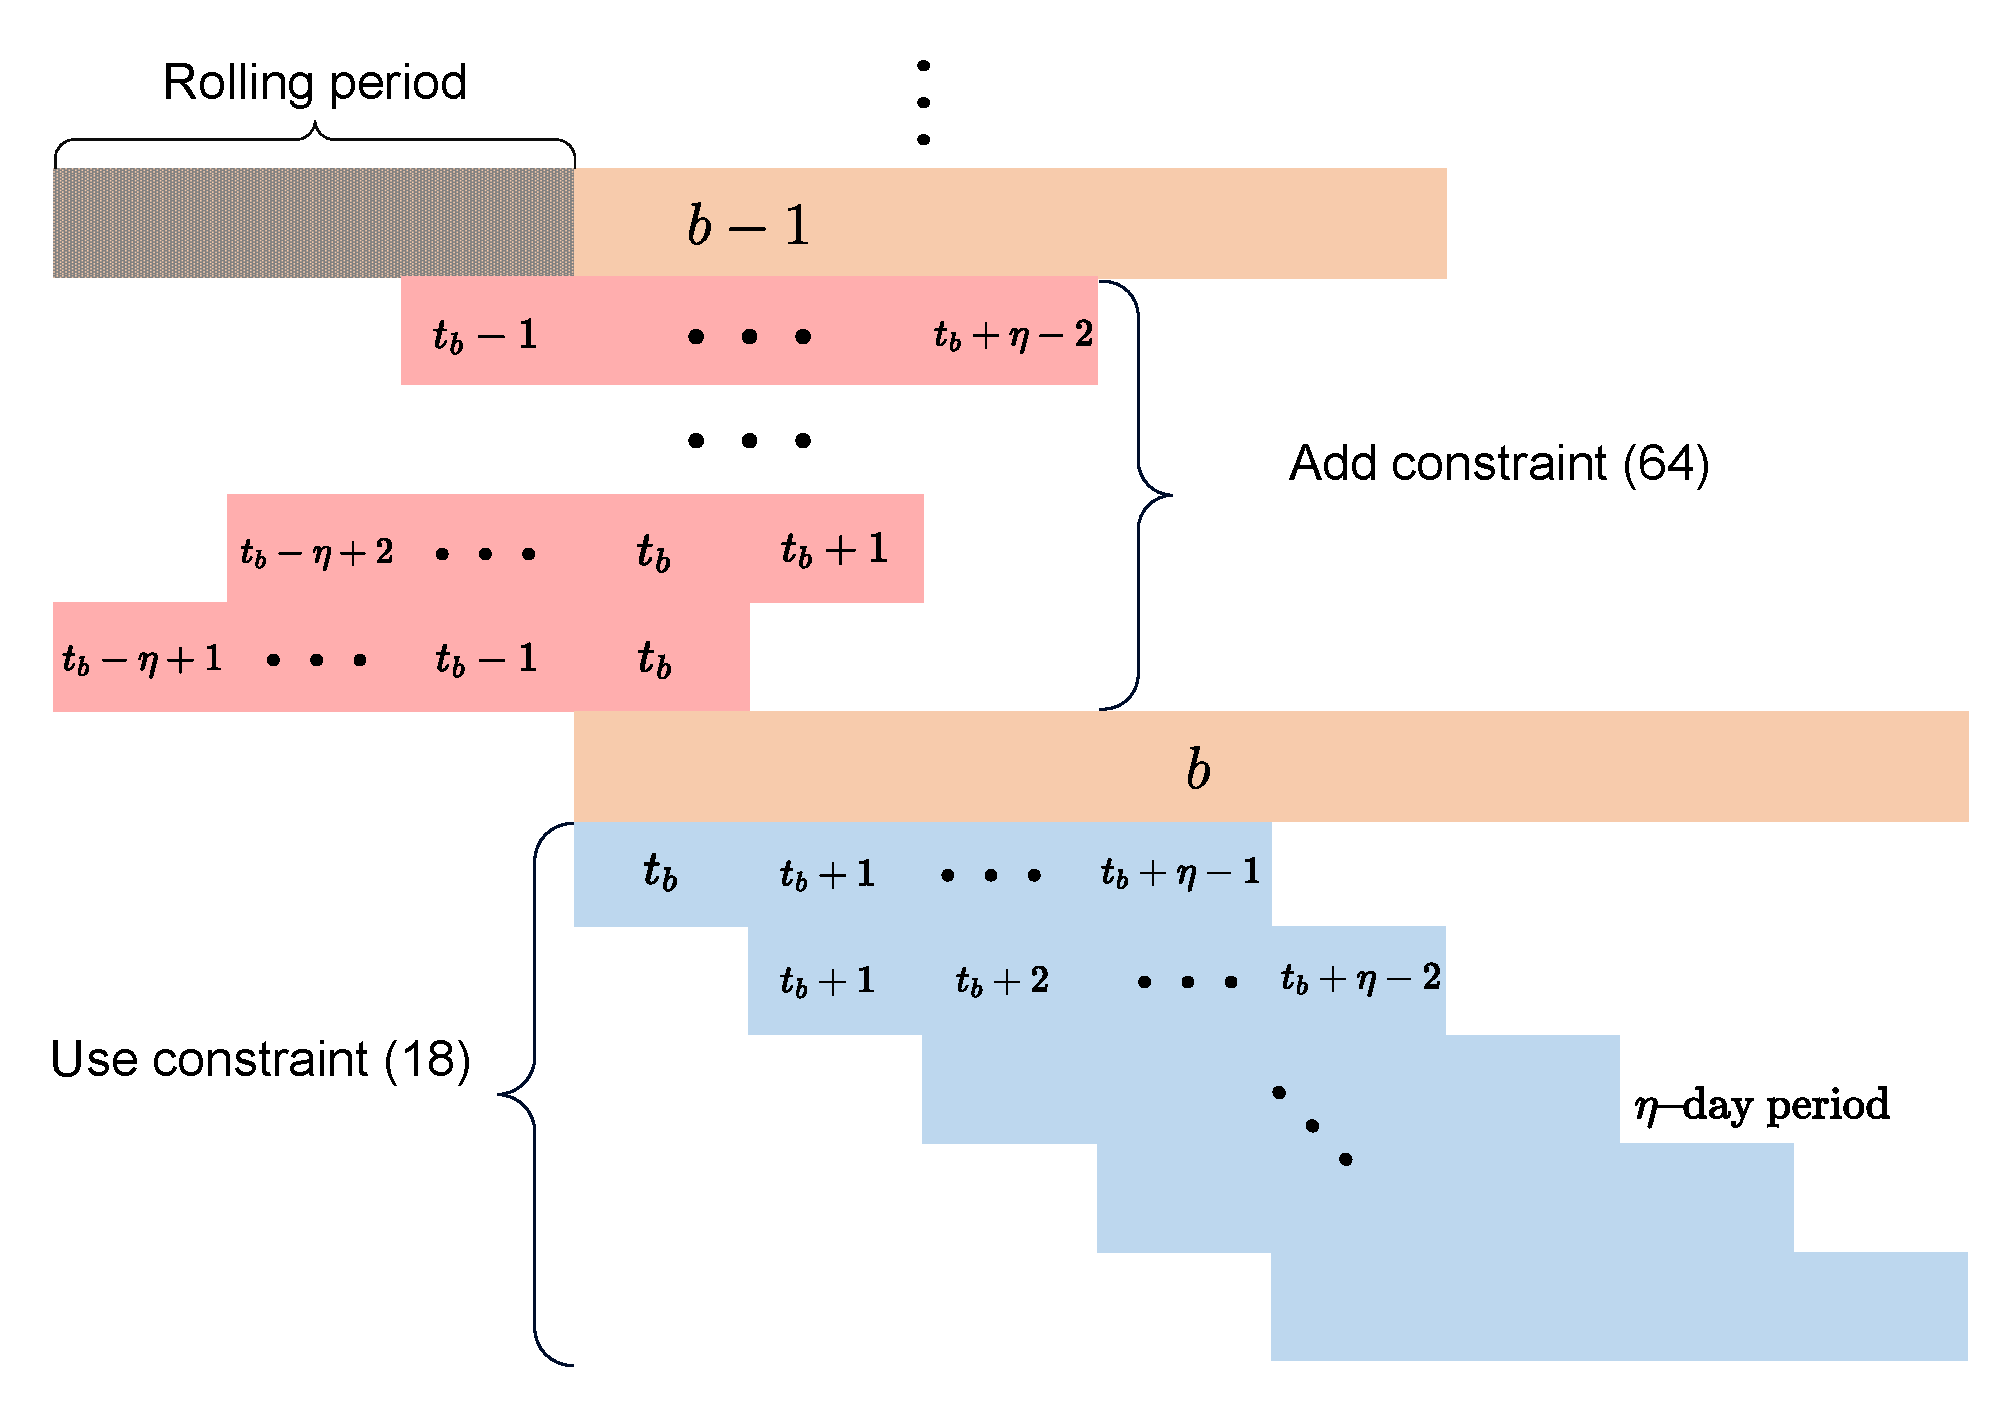
\includegraphics[width=0.7\linewidth]{rh_station_rotation_constraint.pdf} 
    \caption{Diagrammatic explanation of the constraint for aircraft rotation in the temporal decomposition}
    \label{fig:td_stat_rotate}
\end{figure}

Therefore, we add the following constraint to enforce the aircraft rotation constraint and add it to the joint problem for horizon $b$:
\begin{equation}
    \sum_{t'=t - \eta+1}^{t-1} \bar{z}_{ij}^{t'} + z_{ij}^t \leq 1, \quad \forall i \in I, j \in J, t \in \{t_b, t_b +1, \dots, t_b +\eta-2\}, \label{eq:transitionOverTb}
\end{equation}
where $\bar{z}_{ij}^{t'}$ are optimized decisions from the previous horizon, namely horizon $b-1$, and considered as given when solving the problem for horizon $b$.


The effectiveness of the above temporal decomposition approach depends on two key parameters, namely, time horizon $\tau$ and rolling period $\rho$. Using a shorter time horizon reduces computational time but may deteriorate the solution quality due to the limited horizon. In other words, planning is conducted locally within each horizon without considering anything outside of the subject horizon. When the rolling period $\rho$ is small (i.e., the overlap between two time horizons is large), the joint optimization problem is solved more frequently.
This increased frequency, however, results in larger total computation time. When $\rho$ is large, i.e., the overlap between two horizons is small, suboptimality or infeasibility might occur. For example, in the first horizon ranging from Day 1 to Day 10, no maintenance would be scheduled for those tuples with a DTG of 2 on Day 10. This myopic decision is made because of the anticipation that maintenance can be feasibly scheduled on Day 11 in the next horizon for those tuples. However, it might be possible that in the first few days of the second horizon, station access or another capacity parameter is insufficient to accommodate the those tuples, thus causing an infeasibility issue. Even if infeasibility can be avoided, suboptimal planning decisions occur. The likelihood of experiencing infeasibility reduces when the overlap between two horizons increases.

Given the above discussion, we perform a grid search to find the best combination of $\tau$ and $\rho$ to make a good trade-off between the objective value and the computation time. We choose $\tau$ from 20 to 30 days and $\rho$ from 10 to 15 days, with the same step size of five days. 
% Note that optimum tau and rho can differ for each problem (i.e., each problem size)








